\section{Auswertung}
\label{sec:Auswertung}

\subsection{Stabilitätsbedingung}

\begin{figure}[H]
    \centering
    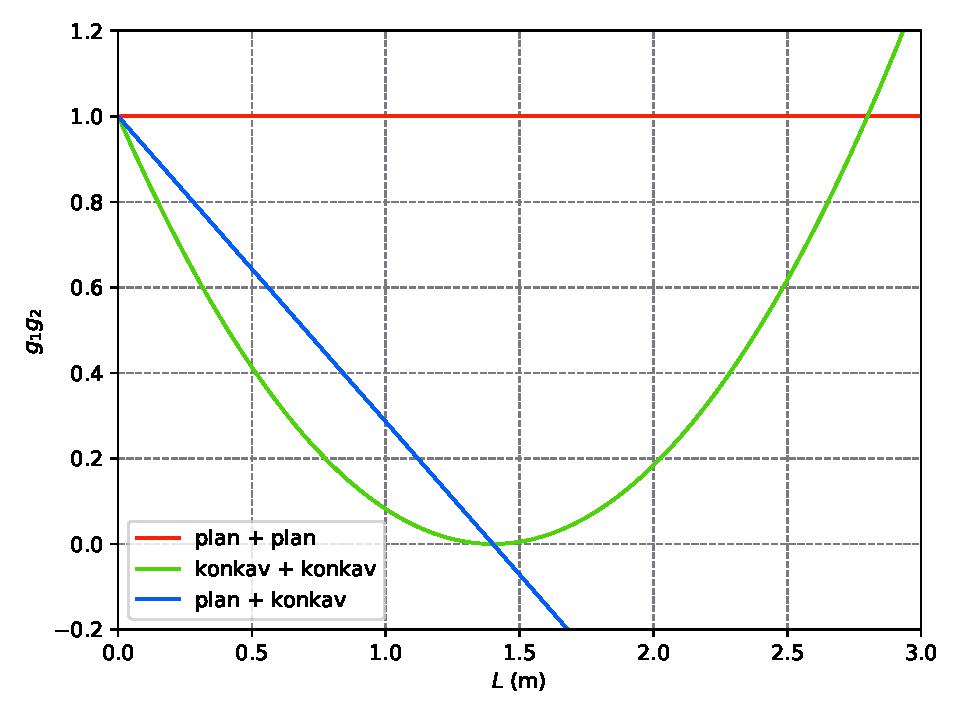
\includegraphics[scale=0.7]{content/g1g2.pdf}
    \vspace{-10pt}
    \caption{Stabilitätsparameter verschiedener Spiegelkonfigurationen planer und konkaver Spiegel mit einem Krümmungsradius
    von $r = \SI{1400}{\milli\meter}$.}
    \label{fig:TEM00}
\end{figure}

\subsection{Transversale Moden}
\subsubsection{TEM$_{00}$-Mode}


\begin{figure}[H]
    \centering
    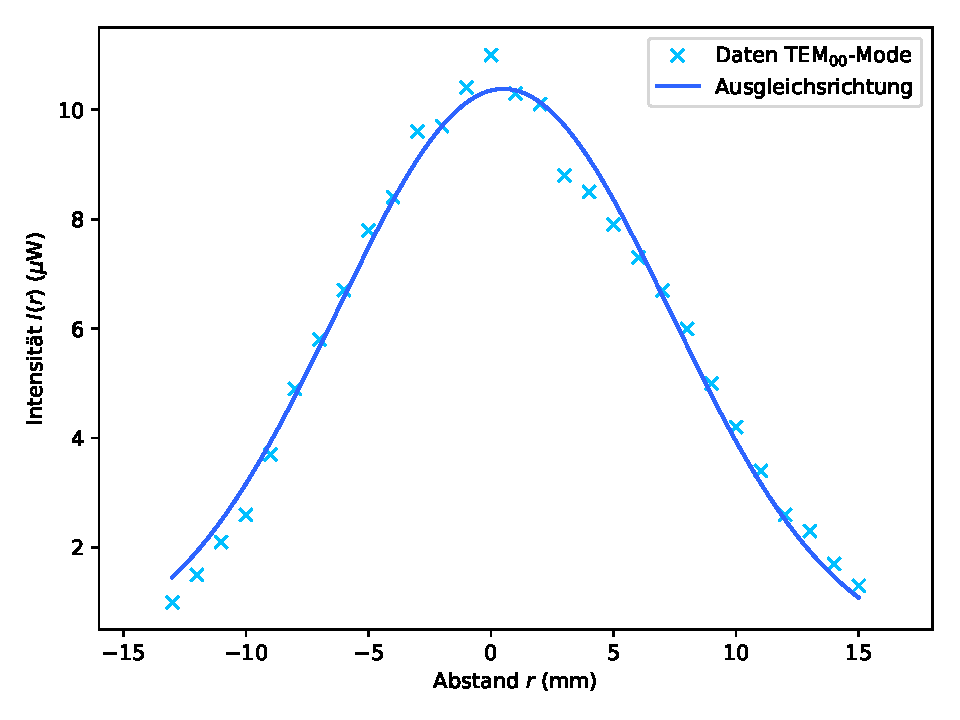
\includegraphics[scale=0.7]{content/TEM00.pdf}
    \vspace{-10pt}
    \caption{Intensitätsverteilung $I(r)$ der TEM$_{00}$-Mode für verschiedene Abstände $r$ von der Modenmitte.}
    \label{fig:TEM00}
\end{figure}

\begin{table}[H]
    \centering
    \caption{Messwerte der Intensität $I(r)$ der TEM$_{00}$-Mode abhängig vom Modenmittenabstand $r$.}
    \label{tab:TEM00}
    \sisetup{table-format=2.1}
    \begin{tabular}{r r | r r | r r}
    \toprule
    $r \;/\; \si{\milli\meter}$ & $I \;/\; \si{\micro\watt}$ & $r \;/\; \si{\milli\meter}$ & $I \;/\; \si{\micro\watt}$
    & $r \;/\; \si{\milli\meter}$ & $I \;/\; \si{\micro\watt}$ \\
    \midrule
        -13 & 1,0 & -3 &  9,6 &  7 & 6,7 \\
        -12 & 1,5 & -2 &  9,7 &  8 & 6,0 \\
        -11 & 2,1 & -1 & 10,4 &  9 & 5,0 \\
        -10 & 2,6 &  0 & 11,0 & 10 & 4,2 \\
         -9 & 3,7 &  1 & 10,3 & 11 & 3,4 \\
         -8 & 4,9 &  2 & 10,1 & 12 & 2,6 \\
         -7 & 5,8 &  3 &  8,8 & 13 & 2,3 \\
         -6 & 6,7 &  4 &  8,5 & 14 & 1,7 \\
         -5 & 7,8 &  5 &  7,9 & 15 & 1,3 \\
         -4 & 8,4 &  6 &  7,3 \\
    \bottomrule
    \end{tabular}
\end{table}

\subsubsection{TEM$_{01}$-Mode}

\begin{figure}[H]
    \centering
    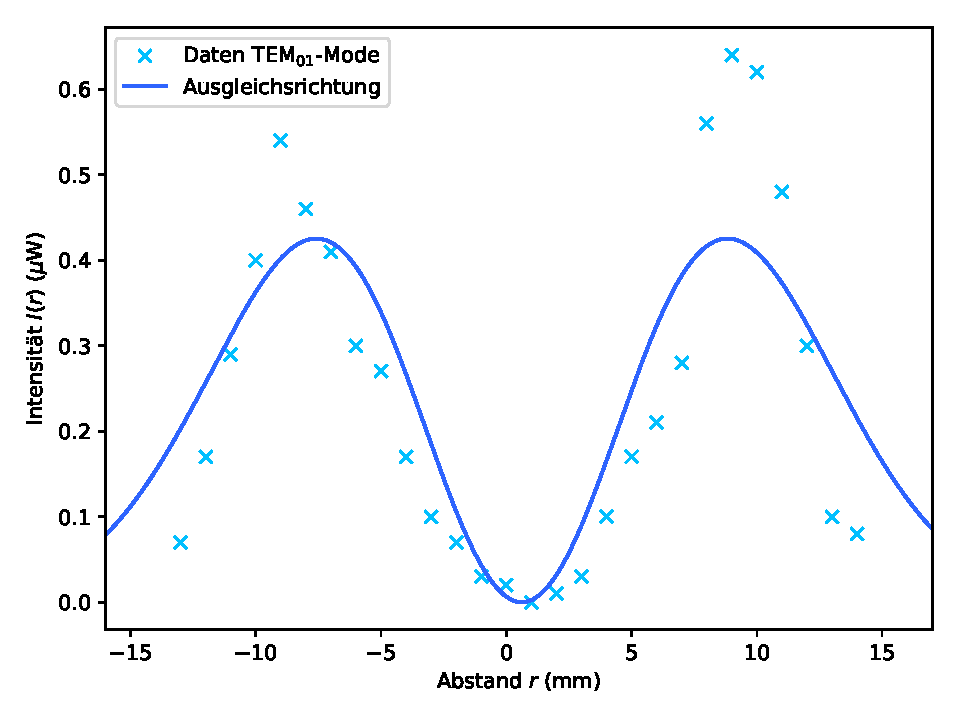
\includegraphics[scale=0.7]{content/TEM01.pdf}
    \vspace{-10pt}
    \caption{Intensitätsverteilung $I(r)$ der TEM$_{01}$-Mode für verschiedene Abstände $r$ von der Modenmitte.}
    \label{fig:TEM01}
\end{figure}

\begin{table}[H]
    \centering
    \caption{Messwerte der Intensität $I(r)$ der TEM$_{01}$-Mode abhängig vom Modenmittenabstand $r$.}
    \label{tab:TEM01}
    \sisetup{table-format=2.1}
    \begin{tabular}{r r | r r | r r}
    \toprule
    $r \;/\; \si{\milli\meter}$ & $I \;/\; \si{\micro\watt}$ & $r \;/\; \si{\milli\meter}$ & $I \;/\; \si{\micro\watt}$
    & $r \;/\; \si{\milli\meter}$ & $I \;/\; \si{\micro\watt}$ \\
    \midrule
        -13 & 0,17 & -3 & 0,20 &  7 & 0,38 \\
        -12 & 0,27 & -2 & 0,17 &  8 & 0,66 \\
        -11 & 0,39 & -1 & 0,13 &  9 & 0,74 \\
        -10 & 0,50 &  0 & 0,12 & 10 & 0,72 \\
         -9 & 0,64 &  1 & 0,10 & 11 & 0,58 \\
         -8 & 0,56 &  2 & 0,11 & 12 & 0,40 \\
         -7 & 0,51 &  3 & 0,13 & 13 & 0,10 \\
         -6 & 0,40 &  4 & 0,20 & 14 & 0,08 \\
         -5 & 0,37 &  5 & 0,27 \\
         -4 & 0,27 &  6 & 0,31 \\
    \bottomrule
    \end{tabular}
\end{table}

\subsection{Polarisation}

\begin{figure}[H]
    \centering
    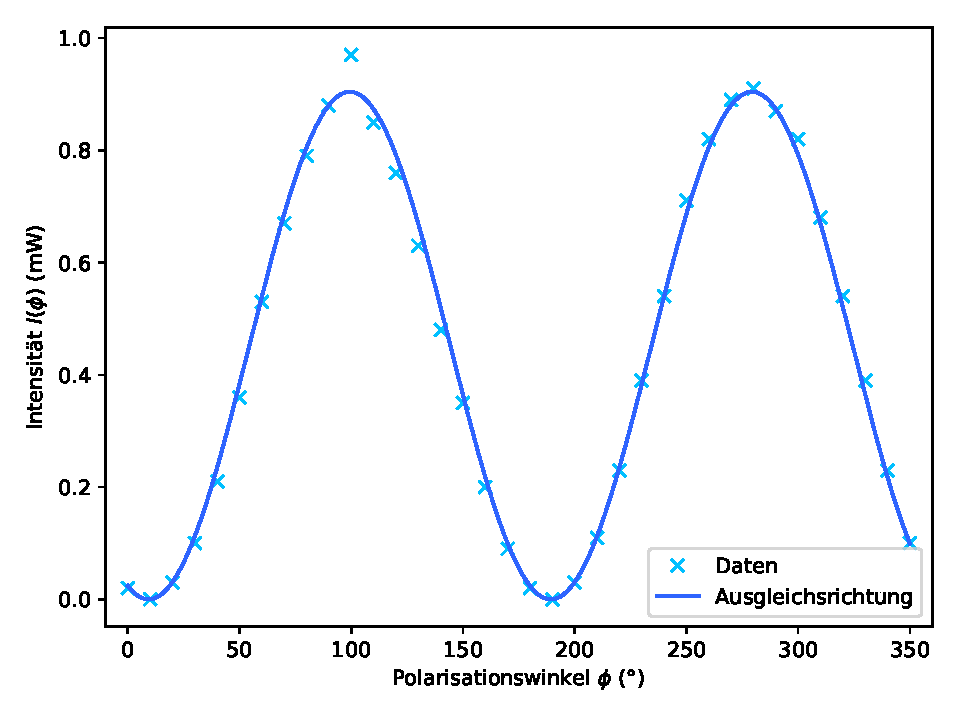
\includegraphics[scale=0.7]{content/pol.pdf}
    \vspace{-10pt}
    \caption{Intensitätsverteilung $I(\phi)$ für verschiedene Polarisationswinkel $\phi$.}
    \label{fig:pol}
\end{figure}

\begin{table}[H]
    \centering
    \caption{Messwerte der Intensität $I(\phi)$ abhängig vom Polarisationswinkel $\phi$.}
    \label{tab:pol}
    \sisetup{table-format=2.1}
    \begin{tabular}{r r | r r | r r}
    \toprule
    $\phi \;/\; \si{\degree}$ & $I \;/\; \si{\milli\watt}$ & $\phi \;/\; \si{\degree}$ & $I \;/\; \si{\milli\watt}$
    & $\phi \;/\; \si{\degree}$ & $I \;/\; \si{\milli\watt}$ \\
    \midrule
         0 & 0,02 & 120 & 0,76 & 240 & 0,54 \\
        10 & 0,00 & 130 & 0,63 & 250 & 0,71 \\
        20 & 0,03 & 140 & 0,48 & 260 & 0,82 \\
        30 & 0,10 & 150 & 0,35 & 270 & 0,89 \\
        40 & 0,21 & 160 & 0,20 & 280 & 0,91 \\
        50 & 0,36 & 170 & 0,09 & 290 & 0,87 \\
        60 & 0,53 & 180 & 0,02 & 300 & 0,82 \\
        70 & 0,67 & 190 & 0,00 & 310 & 0,68 \\
        80 & 0,79 & 200 & 0,03 & 320 & 0,54 \\
        90 & 0,88 & 210 & 0,11 & 330 & 0,39 \\
       100 & 0,97 & 220 & 0,23 & 340 & 0,23 \\
       110 & 0,85 & 230 & 0,39 & 350 & 0,10 \\
    \bottomrule
    \end{tabular}
\end{table}

\subsection{Wellenlänge}

\subsection{Longitudinale Moden}